\subsection{Python Advanced Curve Fitting.}

In a previous lab we fit a line to a set of data in python. That wasn't very hard. But looking at the sample data in the previous graph, it is clear that a straight line won't do.  The data has a definite curve to it. So what equation do we use for our fit? The only equation that makes sense is the equation we developed from our reasoning about RC circuits.

\begin{equation*}
	\Delta V_{C}\left( t\right) =\Delta V_{\max }\left( 1-e^{-\frac{t}{\tau }}\right) \qquad \text{charging}
\end{equation*}

We can use a different python routine to find a curvy equation like this.  We will use the scipy optimize curve\_fit() routine. But we can help the curve\_fit() routine a little by adding in an extra part. Let's code our fit equation like this

\begin{equation*}
	y=A\ast (1-\exp (-B\ast x))+C
\end{equation*}

where we have added a constant $C$. Of course $C$ should be equal to zero or at least should be close to zero because there is no constant term in our theoretical equation. We will need to check for this in our curve fit solution. 

\href{https://raw.githubusercontent.com/rtlines/IntermediateLabPH250/main/Code/user_function_curve_fit_2.py}{Download here}

\lstinputlisting[language=Arduino]{Code/user_function_curve_fit_2.py}

We have to match our variables with the ones we have in our theory equation. Let's compare the equations. 

\begin{eqnarray*}
	y &=&A\ast (1-\exp (-C\ast x))+B \\
	\Delta V_{C}\left( t\right) &=&\Delta V_{\max }\left( 1-e^{-\frac{t}{\tau }}\right) +0
\end{eqnarray*}

We can see that 

\begin{equation*}
	\begin{tabular}{ll}
	                Theory & python \\ 
		$\Delta V_{\max }$ & $A$ \\ 
	                   $0$ & $B$ \\ 
	               $\tau $ & $\frac{1}{\mathtt{C}}$%
	\end{tabular}
\end{equation*}

I suppose we could have just used the theory variables like $\Delta V_max$ in python. you might choose to do that.

\vspace{1in}

Our curve fit might look like this

\begin{figure}[h!]
	\centering
	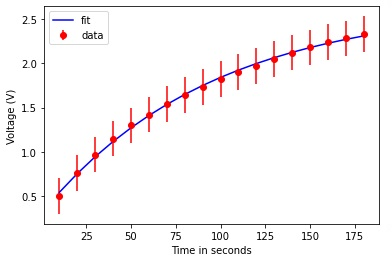
\includegraphics[width=4.561in,height=2.8842in]{RC_circuit_data_with_fit}
\end{figure}

\noindent The program output looks like this:

\begin{verbatim}
	Find a curve fit to a user defined function
	
	The value of A is 2.35419 with standard error of 0.03356.
	The value of B is 0.01051 with standard error of 0.00047.
	The value of C is 0.30913 with standard error of 0.02340.
	
	successful end of program, warning about overflow may follow
\end{verbatim}

If you look at the code you will notice that there is a big difference between the linregress() function and our curve\_fit() function when it comes to the uncertainties in the coefficients. The linregress() function just gave the uncertainteis. But the curve\_fit() function returns a covariance matrix. The diagonal elements of this matrix are our uncertainties on our coefficents -- squared! So we had to take a square root to get the uncertainties.

The curve fit looks nice and that is comforting. For my data, it looks like our capacitor model might be correct, an important thing to check is to see if the curve fit goes through the error bars on all of the data. If it does, it is a good sign that the curve fit might represent the data well.

But now let's go back to our little list of curve fit parameters. We identified 

\begin{equation*}
	\tau =\frac{1}{\mathtt{B}}
\end{equation*}

\noindent and for my data I have 

\begin{equation*}
	\mathtt{B}=0.01051\pm 0.00047
\end{equation*}
\newline

We need units, and looking at the equation we know $\tau $ has units of seconds, so $\mathtt{B}$ must have units of inverse seconds.

\begin{equation*}
	\mathtt{B}=\left( 0.01051\pm 0.00047\right) \frac{1}{\unit{s}}
\end{equation*}

\noindent so we can find a value for $\tau .$ For my data, I have 

\begin{eqnarray*}
	\tau _{measured} &=&\frac{1}{ 0.01051\frac{1}{\unit{s}}} \\
	&=&95.15\,\allowbreak 488\unit{s}
\end{eqnarray*}

Note that we will have to calculate the uncertainty in $\tau .$ I will leave that for an exercise. But I can compare this $\tau _{measured}$ to the $\tau=RC$ value I started with. If they are within each other's error range, this is a powerful confirmation of our capacitor model.


